\section{Fixation du rail magnétique}\label{sec:FixRailMag}
Un problème est survenu lors de la fixation du rail magnétique du moteur sur un des profilés. La partie inférieure du rail est trop courte
pour correctement s'appuyer sur le profilé et le rail rentre dans la rainure lorsqu'il est vissé. La situation est visible sur l'image ci-dessous.

\begin{figure}[H]
    \centering
    \includegraphics[width = 0.4\textwidth]{assets/figures/FixationRailMagProb.png}
    \caption{Illustration du problème de fixation du rail magnétique}
    \label{fig:FixRailMagProb}
\end{figure}

La solution apportée à ce problème est l'utilisation de plaques de fixations placées entre le rail et le profilé. Ceci va permettre de répartir
la charge de chaque côté de la rainure et d'empêcher le rail de pencher en rentrant dans la rainure. Les représentations des deux plaques créées
sont illustrées ci-dessous.

\begin{figure}[H]
    \centering
    \includegraphics[width = 0.7\textwidth]{assets/figures/PlaqueFixation1.svg}
    \caption{Illustration de la première plaque de fixation pour le rail magnétique}
    \label{fig:PlaqueFix1}
\end{figure}

\begin{figure}[H]
    \centering
    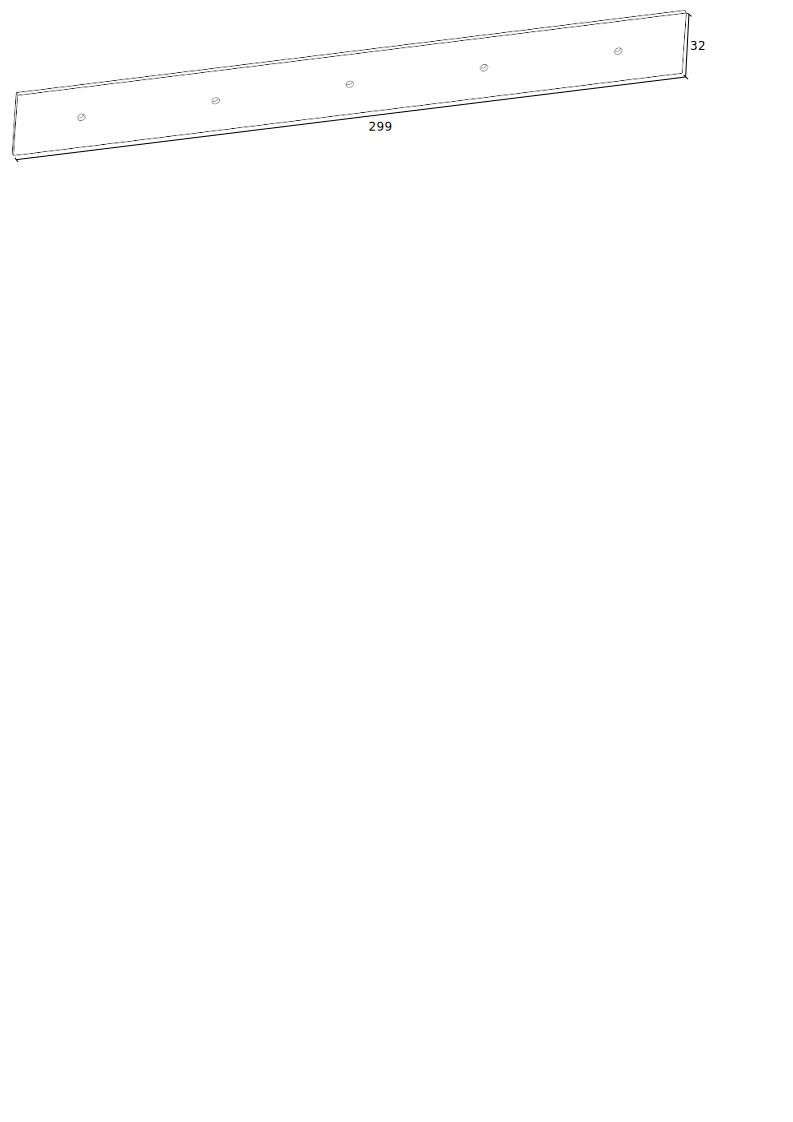
\includegraphics[width = 0.9\textwidth]{assets/figures/PlaqueFixation2.svg}
    \caption{Illustration de la seconde plaque de fixation pour le rail magnétique}
    \label{fig:PlaqueFix2}
\end{figure}

La figure suivante illustre la solution appliquée et comment elle résout le problème.

\begin{figure}[H]
    \centering
    \includegraphics[width = 0.4\textwidth]{assets/figures/FixationRailMagSol.png}
    \caption{Illustration de la solution de fixation du rail magnétique}
    \label{fig:FixRailMagSol}
\end{figure}

Cependant, cette modification éloigne le rail magnétique de 2~mm du chariot. Il faut donc modifier la pièce de liaison au moteur pour la ralonger
de 2~mm aussi. Le support de la tête de lecture de la règle linéaire est aussi décalée afin de maintenir la position de la tête de lecture.

\section{Jeu dans le guidage linéaire}\label{sec:JeuGuidage}
En faisant des déplacements à la main sur le moteur on se rend compte que le mouvement n'est pas aussi fluide que voulu. La raison de ce mouvement
est le jeu présent entre le rail de guidage linéaire et le chariot. La figure suivante permet d'illustrer les explications qui vont suivre.

\begin{figure}[H]
    \centering
    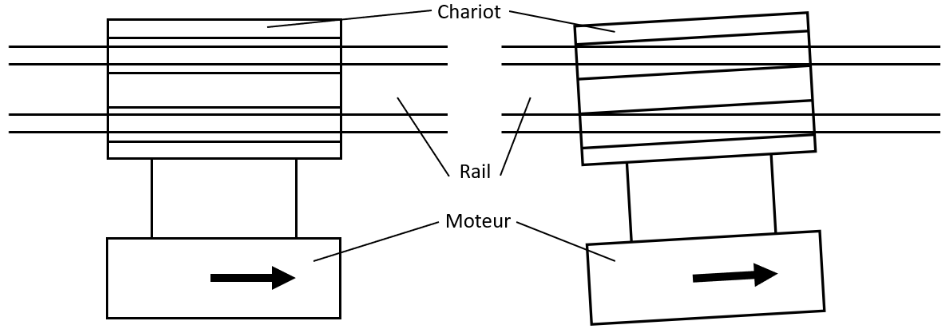
\includegraphics[width = 0.8\textwidth]{assets/figures/ImprevuJeuRail.svg}
    \caption{Illustration des effets du jeu sur le rail}
    \label{fig:JeuRail}
\end{figure}

Le moteur génère une force horizontale sur la partie mobile qui se trouve à une certaine distance du rail de guidage ce qui engendre un moment.
Ce moment fait pivoter le système car rien ne l'empêche étant donné la présence du jeu. Cette rotation diminue la surface de contact ce qui
augmente la force d'appui ce qui va augmenter à son tour la force de frottement.\\

La solution la plus simple à ce problème est de graisser le rail afin de réduire les frottements. Cette solution permet d'obtenir un mouvement
fluide mais ne répond pas aux autres problèmes éventuels que ce jeu pourrait engendrer comme par exemple une lecture de position linéaire
erronnée dû à la précision nécessaire entre la position de la tête de lecture et la règle de mesure.\\

La deuxième solution serait d'utiliser un autre rail avec une précontrainte ce qui éliminerait le jeu. Parmis les rails proposés dans le
chapitre \ref{sec:CatSol}, le rail de chez Hiwin \cite{Hiwin} utilise des billes et peut être précontraint. Il possède même une mesure de
position intégrée ce qui faciliterait et augmenterait la précision de la mesure de position.\\

Dans le cas de ce projet, l'acquisition d'un nouveau rail n'est pas envisageable par manque de temps. L'option du lubrifiant sera utilisé pour
essayer de faire déplacer le pendule pendant la période d'août.

\section{Support chaîne porte-câbles}\label{sec:ProbChaine}
En montant la chaîne sur son support on s'aperçoit très vite que le support n'est pas suffisant et que la chaîne descend de 15~cm au plus bas.
La solution à ce problème est d'ajouter un autre support sur la course de la chaîne. Le rail d'aimants du moteur linéaire possède des taraudages
M5 sur le dessous. Le support peut donc être imprimé en 3D pour venir se fixer en dessous du rail magnétique et venir supporter la châine porte-câbles.
L'image suivante illustre la solution.

\begin{figure}[H]
    \centering
    \includegraphics[width = 0.45\textwidth]{assets/figures/ProbChaine.svg}\hfill
    \includegraphics[width = 0.45\textwidth]{assets/figures/SolChaine.svg}
    \caption{Illustration du problème et de la solution au problème de chaîne porte-câbles}
    \label{fig:SolChaine}
\end{figure}

\section{Combinaison de capteur non valide}\label{sec:ProbCapt}
Lors du paramètrage de l'EPOS4 pour le moteur et les capteurs, la combinaison de capteurs utilisée pour le projet n'a pas été acceptée comme
valide pour faire fonctionner le contrôleur. En effet comme on peut le voir sur le tableau ci-dessous extrait de la \textit{datasheet} du contrôleur, un
capteur incrémental digital et un capteur incrémental analogique ne sont pas suffisant pour pouvoir utiliser la carte.

\begin{figure}[H]
    \centering
    \includegraphics[width = 0.7\textwidth]{assets/figures/TableauCapteur.png}
    \caption{Extrait de la \textit{datasheet} de l'EPOS4 sur les combinaisons de capteurs utilisable}
    \label{fig:TableauCapteur}
\end{figure}

Deux options sont possibles pour remédier à ce problème. La première consiste à remplacer un des capteurs par un capteur SSI absolu ce qui
requiert de chercher un capteur adéquat, attendre qu'il soit livré et modifier la structure pour pouvoir l'accueillir. La seconde solution
serait d'installer des capteurs à effet Hall à côté du glider du moteur. Etant donné du peu de temps restant pour la complétion du projet le
choix de solution s'est porté sur la seconde proposition. L'image suivante illustre comment le support se placera sur le moteur.\\

\begin{figure}[H]
    \centering
    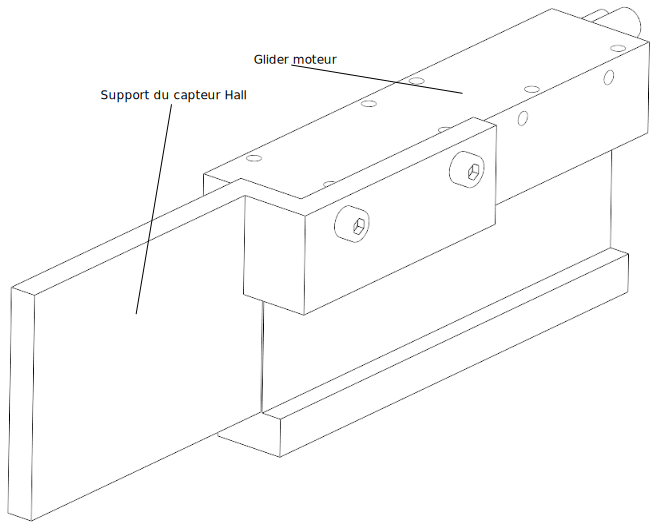
\includegraphics[width = 0.7\textwidth]{assets/figures/SolCapt.svg}
    \caption{Illustration du montage du support sur le glider du moteur}
    \label{fig:SolCapt}
\end{figure}

Pendant le mois d'août, la démarche suivante devra être appliquée pour venir à bout du problème. Premièrement, il faut commander un circuit de
mesure utilisant des capteurs à effet Hall. Ensuite, dessiner et imprimer en 3D un support pour le capteur qui peut se monter sur le côté du
glider moteur. Enfin, câbler le connecteur pour sondes à effet Hall pour pouvoir se connecter sur le connecteur X4 de l'EPOS4.